

\section{ApoCo-GUI Gestaltung}

Die grafischen Elemente, wie Hintergrundbilder, farbige Buttons, Splashscreen, Farbgebung und das Logo,
sind mit einer Software f\"ur Bildbearbeitung und Illustration,
speziell f\"ur die Android-Anwendung designet.
Soweit es die Funktionalit\"at der einzelnen Activity zul\"asst, sind alle Activities identisch strukturiert.
Sie besitzen in diesem Fall immer die Elemente \emph{Header, Title, Body} und \emph{Footer}.
Das Einhalten der Struktur soll durch ein einheitliches Layout eine angenehme und einfache Bedienung der Software erm\"oglichen.
Die Abbildung 4.12 veranschaulicht und benennt die Hauptstrukturelemente einer Activity anhand der Start-Activity der ApoCo-Anwendung.\\

\begin{figure}[h]
  \centering
  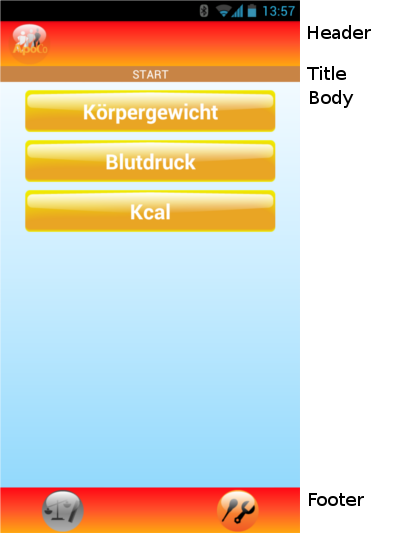
\includegraphics[scale=0.5]{screenshots/kapitel4/gui/activity_struktur.png}
  \caption{Start-Activity als Beispiel f\"ur Strukturierung}
  
\end{figure}

Die Strukturelemente haben jeweils eine eigene Funktion.
\begin{itemize}
 \item Header:\\
 Im \emph{Header} ist immer das ApoCo-Logo und wenn notwendig, ein \emph{Back-Button} angebracht.

 \item Title:\\
 Der \emph{Title} Bereich informiert den Benutzer auf welcher Activity er sich im Augenblick befindet.
 \item Body:\\
 Im \emph{Body} sind Interaktionselemente oder weitere notwendige Informationen der aktuellen Activity angebracht.
 Das k\"onnen Buttons zum Ansto\ss{}en von Messvorg\"angen oder ListViews sein.
 Eine ListView informiert den Benutzer \"uber alle bereits verzeichneten Messungen in der entsprechenden Activity.
 \item Footer:\\
 Am Ende der Activity ist der \emph{Footer}.
 Er beinhaltet Buttons, mit denen man in die Bereiche zum Ger\"ate-Koppeln, Sprung zur Start-Activity und zur 
 Server-Konfiguration gelangt. 
\end{itemize}


\subsection{Bedienelemente}

\subsubsection{Zur\"uck-Funktion}

Der Back-Button ist eines von mehreren M\"oglichkeiten, mit der ein Benutzer zu der vorherigen Activity zur\"uckkehren kann.
Einige davon haben lediglich die Funktion \emph{zur\"uck und Daten verwerfen} und andere wiederum 
\emph{zur\"uck und Daten speichern}.
Die Abbildung 4.13 veranschaulicht einen \emph{Header} mit \emph{Back-Button}.\\

\begin{figure}[h]
  \centering
  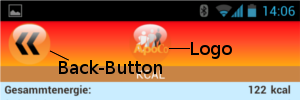
\includegraphics[scale=0.5]{screenshots/kapitel4/gui/header_backbtn.png}
  \caption{Header einer Activity mit \emph{Back-Button}}
  
\end{figure}

Die Abbildung 4.14 zeigt die Activity f\"ur Blutdruckmessung.
Mit Buchstaben sind hier alle M\"oglichkeiten der Software gekennzeichnet, die zur\"uck in die vorherige Activity f\"uhren.\\


\begin{figure}[h]
  \centering
  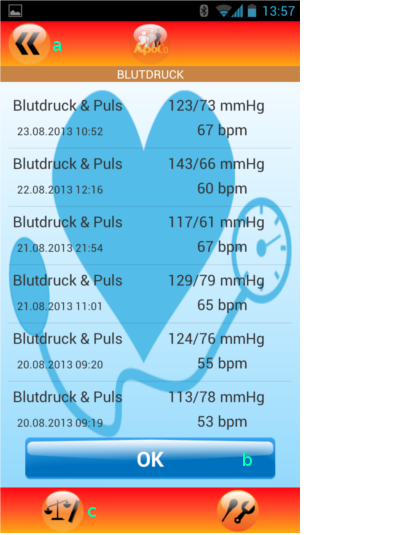
\includegraphics[scale=0.5]{screenshots/kapitel4/gui/back_btns.png}
  \caption{Zur\"uck-M\"oglichkeiten einer Activity}
  
\end{figure}


\begin{itemize}
 \item a) \emph{Back-Button}, Daten werden nicht gespeichert, zur\"uck zur vorherigen Activity. 
 \item b) \emph{OK-Button}, Daten werden gespeichert, anschlie\ss{}end zur\"uck zur vorherigen Activity.
 \item c) Sprung zur \emph{Start-Activity}, Daten werden nicht gespeichert. 
\end{itemize}

Neben einer Softwarem\"oglichkeit ist auch der Hardware-Button des Smartphones implementiert.
In der Abbildung 4.15 ist der Hardware-Button mit einem roten Kreis gekennzeichnet.
Hier findet kein Speichern der Daten statt.
Befindet man sich in der \emph{Start-Activity}, beendet ein Dr\"ucken auf die Hardware-Taste die ApoCo-Anwendung.\\

\begin{figure}[h]
  \centering
  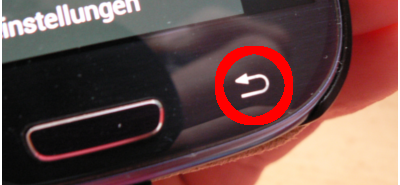
\includegraphics[scale=0.5]{screenshots/kapitel4/gui/hd_backbtn.png}
  \caption{Zur\"uck mit einem dem Hardware-Button des Smartphones}
  
\end{figure}

\subsubsection{Ger\"ateverwaltung}

In der Abbildung 4.16 ist der Button zur Ger\"ateverwaltung abgebildet.
Mit diesem Button gelangt man in den Bereich der Android-Anwendung, in welchen 
Messger\"ate gekoppelt und Servereinstellungen vorgenommen werden k\"onnen.

\begin{figure}[h]
  \centering
  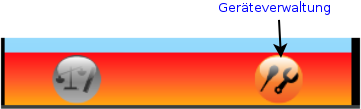
\includegraphics[scale=0.5]{screenshots/kapitel6/android/devices.png}
  \caption{Ger\"ateverwaltung}
  
\end{figure}

Die Abbildung 4.17 veranschaulicht anschlie\ss{}end die Activity der Ger\"ateverwaltung.
Hier wird \"uber Radio-Buttons eine Messung ausgew\"ahlt und \"uber eine der Koppelungsfunktionen
die externe Hardware verbunden.
Ob hier das Koppeln als Server oder Client gew\"ahlt wird, ist von dem externen Messsensor abh\"angig.\\

\begin{figure}[h]
  \centering
  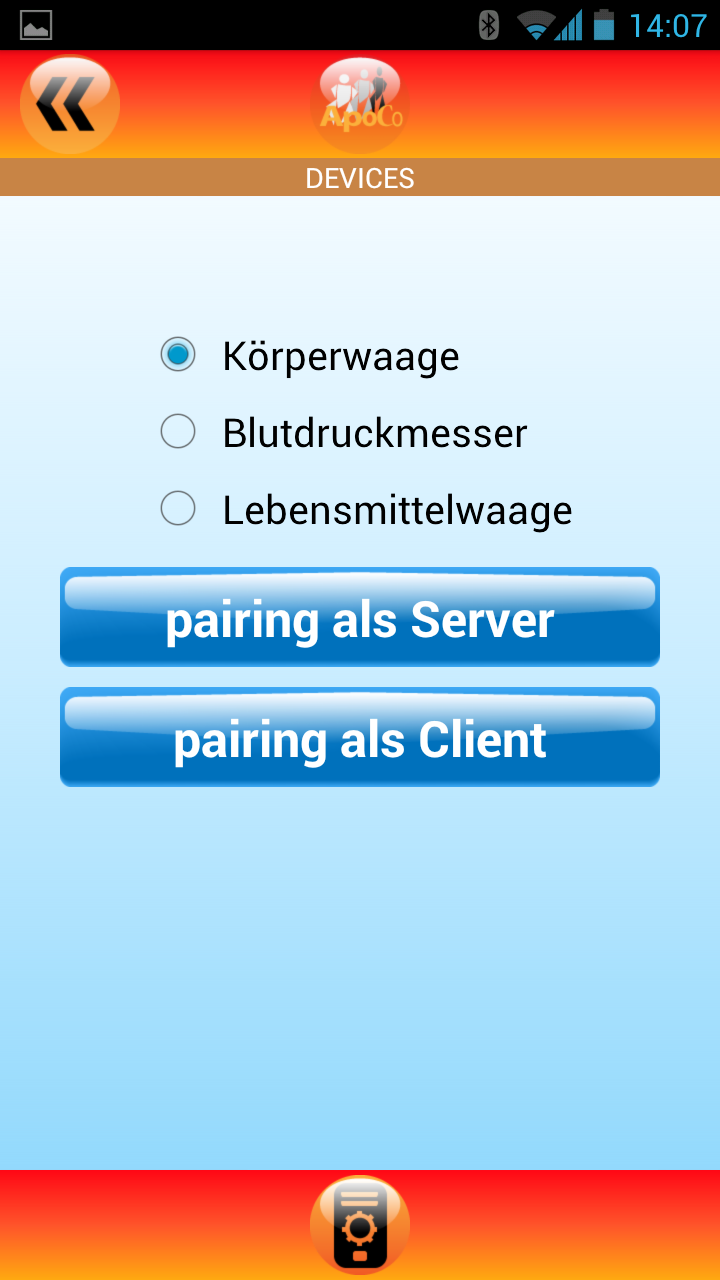
\includegraphics[scale=0.2]{screenshots/kapitel4/pairing.png}
  \caption{Koppelungsactivity}
  
\end{figure}

Im \emph{Footer}-Bereich der Abbildung 4.17 ist auch der Button f\"ur die Serverkonfiguration zu finden.
Die Serverkonfiguration wird mittels einer Activity realisiert, die sich allerdings im \emph{Dialog-Stil} pr\"asentiert.
Diese Aktivity wird in der Abbildung 4.18 veranschaulicht und das Listing 4.17 erl\"autert, 
wie man eine Activity \"uber das \emph{AndroidManifest} als Dialog erscheinen l\"asst.\\

\begin{figure}[h]
  \centering
  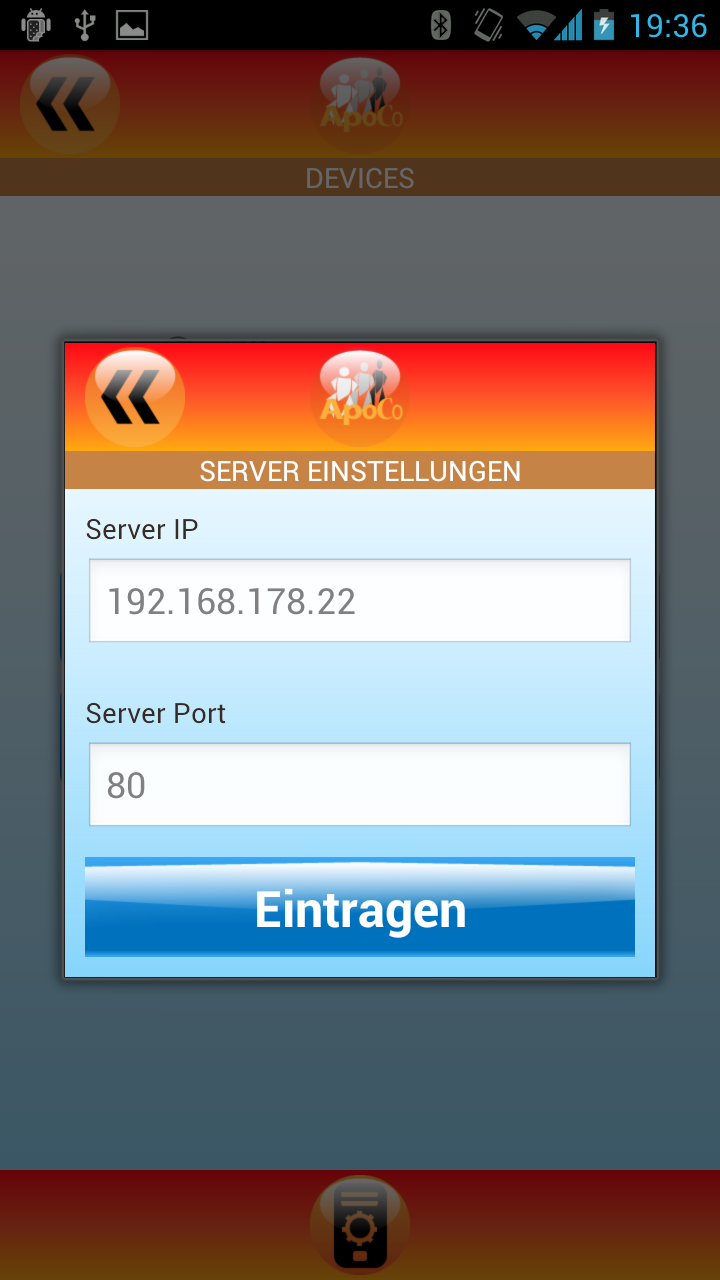
\includegraphics[scale=0.2]{screenshots/kapitel4/server_einstellungen.png}
  \caption{Serverkonfiguration}
  
\end{figure}

 \begin{lstlisting}[caption={Activity als Dialogfenster erscheinen lassen}]
 <activity
   android:name="com.janas.apoco.activity.ActivityServerOptions"
   //die zweite Zeile l\"asst die Activity als Dialog erscheinen
   android:theme="@android:style/Theme.Dialog" >
</activity>
\end{lstlisting}


\subsection{Activity-Wechsel mit Animation}

Der Wechsel von einer Aktivity zur anderen wird mit Animationsskripten gemacht.
Dabei wird die erste Activity zum Bildrand rausgezogen und die zweite Activity ins Bild hineingezogen.
Handelt es sich um den Wechsel zu einer Activity, die sich auf eine Parametrierung der Software bezieht, 
so verl\"auft die Animation von unten nach oben.
Wechselt man aber zur einer Messung, so verl\"auft die Animation von rechts nach links.
Eine vollst\"andige Animation besteht immer aus den zwei Teilen \emph{Eingangs-} und \emph{Ausgangs}-Animation.
Die Animationen sind im Odrner \emph{/res/anim/} in \emph{XML}-Dateien abgelegt.
Das Listing 4.18 veranschaulicht die Definition einer Animation und wie man sie f\"ur den Wechsel der Activities nutzt.\\

\begin{lstlisting}[caption={Animation zum Verlassen einer Activity}]
//rigt_side_in.xml
<?xml version="1.0" encoding="utf-8"?>
<set xmlns:android="http://schemas.android.com/apk/res/android" 
    android:interpolator="@android:anim/accelerate_decelerate_interpolator" >    
    <translate
        android:fromXDelta="100%p"
        android:toXDelta="0"
        android:duration="500"/>    
</set>
//Anwendung der Animation in einer Activity
finish();
overridePendingTransition(R.anim.left_side_in, R.anim.left_side_out);
\end{lstlisting}

Im Listing 4.18 ist ein Beispiel einer Animation f\"ur die reinkommende Activity zu sehen.
Durch den Aufruf der Methode \emph{overridePendingTransition()} wird eine Animation gestartet.
Diese Methode hat jedes Objekt vom Typ \emph{Activity}.
Sie muss zum Aufrufen \"uberschrieben werden.
Der Aufruf muss anschlie\ss{}end immer nach einer Methode erfolgen, welche f\"ur das Schlie\ss{}en einer Activity zust\"andig ist.
Das sind die Methoden \emph{finish()} und alle aus der Familie \emph{startActivity...()}.
Die Abbildung 4.19 zeigt zwei Screenshots mit jeweils einer Animation.
Bei der ersten ist der Wechsel in eine Messung zu sehen und in der zweiten zum Koppelungsvorgang.\\

\begin{figure}[h]
  \centering
  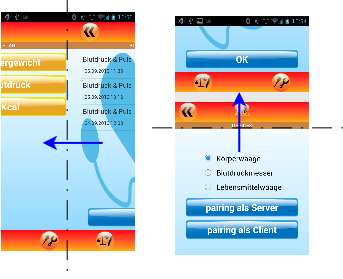
\includegraphics[scale=0.7]{screenshots/kapitel6/android/animation_richtung.png}
  \caption{\"Ubergangsanimation}
  
\end{figure}

\subsection{Views und Struktur der gegenseitigen Aufrufe}

In der Abbildung 4.20 ist die gesamte Viewschicht der Android-Anwendung veranschaulicht.
Die gro\ss{}en blauen Makierungen identifizieren die Views.
Wird ein Button gedr\"uckt, weist eine kleine blaue Makierung darauf hin, welche View als n\"achstes ge\"offnet wird.
Eine Ausnahme ist die View \emph{Splashscreen (s1)} und der Barcodescanner \emph{(b2)}.
Der \"Ubergang von Splashscreen zur Anmelde-View \emph{(a1)} geschieht \"uber einen Timer.
Ist der Timer abgelaufen, so startet der \"Ubergang automatisch.
Im Fall der Barcodescanner-View h\"angt der \"Ubergang davon ab,
ob nach dem Scan der Barcode in der Datenbank f\"ur Lebensmittel gefunden wurde oder nicht.
War die Suche erfolgreich, dann geht es mit der View \emph{(k3)} weiter.
Ist die Suche fehlgeschlagen, findet der \"Ubergang zur View \emph{(k2)} statt.\\

\begin{figure}[h]
  \centering
  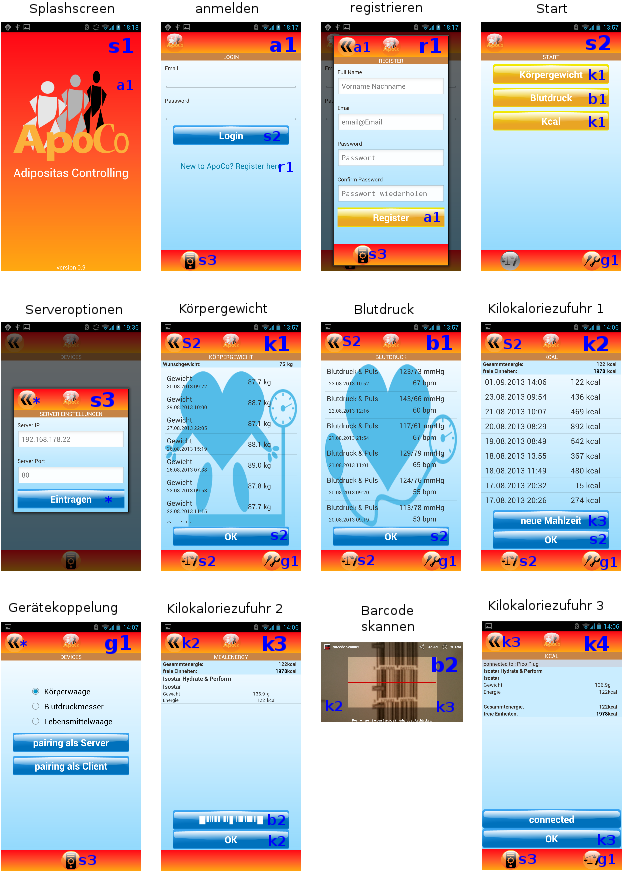
\includegraphics[scale=0.6]{diagramme/kapitel6/android/activity_map.png}
  \caption{Darstellung aller Activities}
  
\end{figure}

Um den Zusammenhang der Views besser darzustellen, 
zeigt die Abbildung 4.21 ein Zustandsdiagramm.
Dieses Zustandsdiagramm stellt die Beziehungen der Views untereinander dar.
Damit die Komplexit\"at des Diagramms \"uberschaubar bleibt,
wurde auf die Modellierung der Buttons f\"ur \emph{akzeptierende} und \emph{ablehnende} Aktionen verzichtet.
Im Diagramm sind nur die m\"oglichen \"Uberg\"ange zwischen den Views dargestellt.
Die Bezeichner der Zust\"ande im Diagramm entsprechen den Makierungen in der Abbildung 4.20, welche die Views identifizieren.
Zus\"atzlich sind die \"Ubergangspfade beschriftet und nummeriert.
Die Beschriftungen sagen aus, welche Aktion auf diesem Pfad vollzogen wird.
Die Nummerierungen bilden eine Hierarchie und sollen aufzeigen auf welche Weise ein Pfad verfolgt werden darf.
Es ist nur erlaubt einem wegf\"uhrenden Pfeil zu folgen, wenn der Pfad zuvor die gleiche Nummerierung hatte,
oder seine Nummerierung dem Folgepfeil als Pr\"afix vorangestellt ist.
Gelangt man \"uber einen Pfad zu einem verzweigenden Zustand,
dann wird die Nummerierung des letzten Pfeils
zum Pr\"afix der n\"achsten Pfade.\\
Betrachtet man den Zustand \emph{(r1)} in Abbildung 4.21.,
so ist es m\"oglich von \emph{(r1)} in den Zustand \emph{(s3)} hin und wieder zur\"uck zu wechseln.
Da keiner der restlichen Pfeile von \emph{(s3)} aus mit der 1 im Pr\"afix nummeriert ist, 
ist es beispielsweise nicht erlaubt von \emph{(s3)} nach \emph{(k4)} oder den \"ubrigen Zust\"anden zu wechseln.\\



\begin{figure}[h]
  \centering
  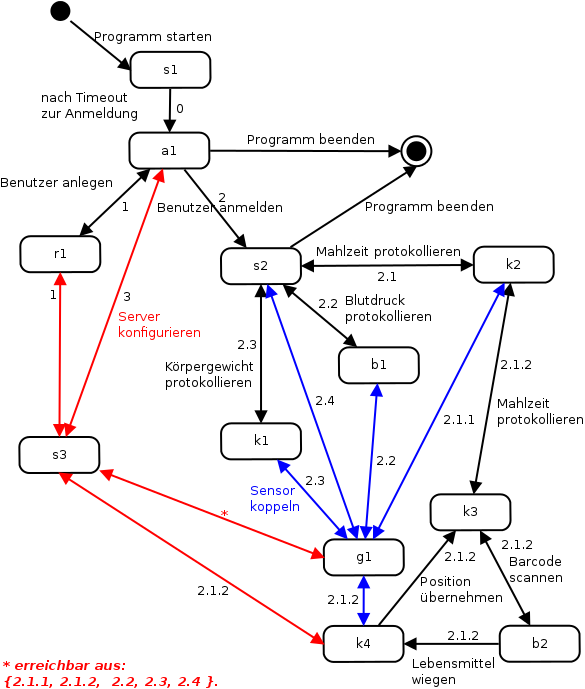
\includegraphics[scale=0.6]{diagramme/kapitel6/android/zustand_dialog_beziehung.png}
  \caption{Zustandsdiagramm f\"ur Beziehungen der gegenseitigen Aufrufe}
  
\end{figure}
